Convolutional neural network, Autoencoder, embedding, optimizers, regularization, descriptions of how each layer works.

Convolutional neural networks (CNNs) capture nonlinear rela- tionships over large areas of images, resulting in vastly improved performance for image recognition tasks as compared to classical machine learning methods

TODO cite Oukomol

\begin{figure}[htb]
	\begin{center}
		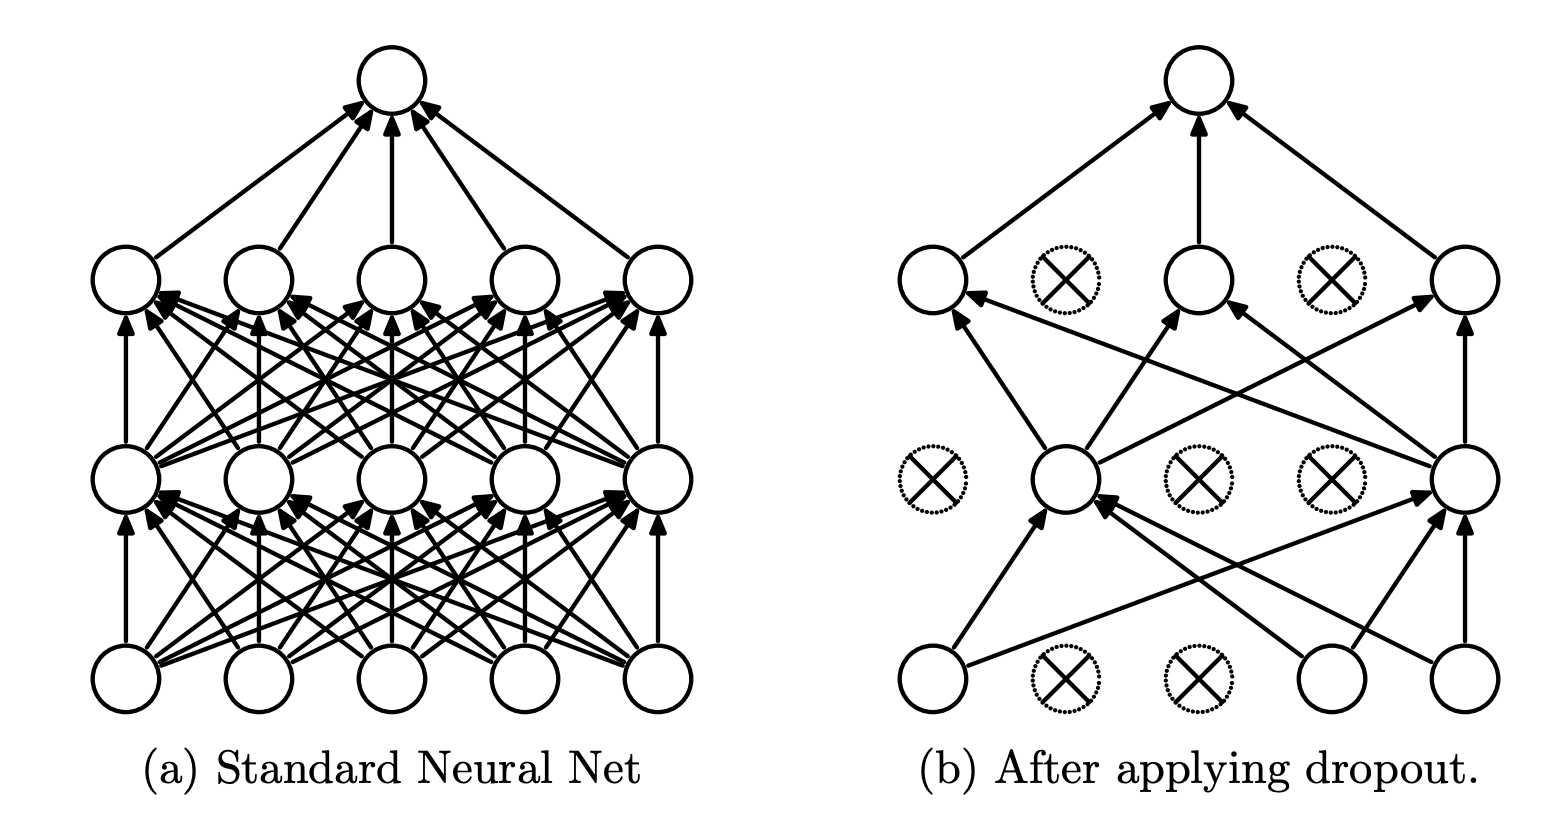
\includegraphics[width=0.8\linewidth]{bilder/dropout.png}
		\caption{Dropout}\label{fig:dropout}
	\end{center}
\end{figure}